\section{Results}
\subsection{Fleet warm start halves local experimentation}
Figure~\ref{fig:convergence} shows oracle-relative regret versus new target-local experiments. Both fleet-informed methods improve markedly faster than independent BO, while global and dynamics-weighted warm start remain nearly indistinguishable.

\begin{figure*}[t]
\centering
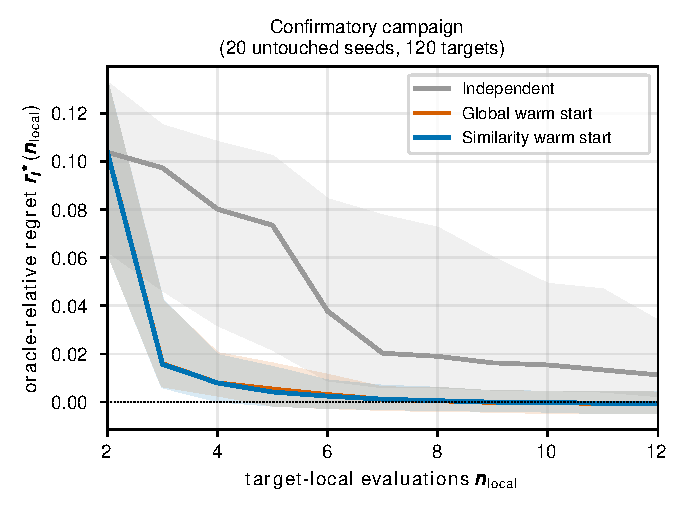
\includegraphics[width=0.98\textwidth]{figures/fig3_confirmatory_convergence.pdf}
\caption{Pre-registered confirmatory convergence on 20 untouched fleet seeds and 120 held-out targets. Mature-fleet warm start accelerates target-local controller calibration from the first BO iterations; dynamics weighting and unweighted pooling exhibit essentially identical convergence.}
\label{fig:convergence}
\end{figure*}

Independent BO requires on average 6.63 local experiments to reach within 5\% of the client-specific oracle, compared with 3.07 for global fleet warm start, a 54\% reduction. The standard deviation decreases from 3.76 to 0.81, showing that warm start primarily removes the long tail of difficult cold-start targets. The paired seed-level global-minus-independent difference is $-3.567$ experiments, with 95\% bootstrap CI $(-4.908,-2.333)$ and Wilcoxon $p=0.0005$. The result is consistent across all three vehicle families.

\begin{table}[t]
\centering
\caption{Confirmatory target-local sample efficiency.}
\label{tab:main_results}
\scriptsize
\resizebox{\columnwidth}{!}{%
\begin{tabular}{@{}lccccc@{}}
\toprule
Method & Mean & Median & Std. & $P(\Nfive\le3)$ & $P(\Nfive\le5)$\\
\midrule
Independent & 6.633 & 6.0 & 3.762 & 0.283 & 0.425\\
Global warm start & 3.067 & 3.0 & 0.807 & 0.767 & 0.992\\
Dynamics weighted & 3.058 & 3.0 & 0.770 & 0.758 & 1.000\\
\bottomrule
\end{tabular}%
}
\end{table}

After only three local experiments, 76.7\% of globally warm-started targets reach the 5\% criterion, compared with 28.3\% under independent BO. After five experiments, the rates are 99.2\% and 42.5\%, respectively (Fig.~\ref{fig:n5}).

\begin{figure*}[t]
\centering
\includegraphics[width=0.98\textwidth]{figures/fig4_n5pct_summary.pdf}
\caption{Target-local experiment count required to reach within 5\% of the client-specific oracle. Fleet warm start approximately halves the mean commissioning effort and largely removes the difficult-client tail.}
\label{fig:n5}
\end{figure*}

\subsection{Dynamics-aware weighting adds no measurable benefit}
On the confirmatory data, dynamics-weighted warm start is statistically indistinguishable from global pooling. The paired seed-level mean difference in $\Nfive$ is $-0.008$ experiments with 95\% CI $(-0.058,+0.033)$ and Wilcoxon $p=0.706$. The secondary early-window $\AURCstar$ gives the same conclusion, with difference $-0.0005$, CI $(-0.0050,+0.0041)$, and $p=0.936$.

The null result is structural rather than numerical. The weighting strongly attenuates some cross-family observations and can change acquisition decisions, but the calibration objective is far more invariant than the plant dynamics: all evaluated client pairs have $\rho_{ij}^{J}\ge0.95$. A development-stage coverage experiment also limited the mature prior to nine peers and varied same-family sources from five to zero. Dynamics weighting did not outperform global pooling at any coverage level; even same-family-only source selection was slightly worse than retaining all observations. Figure~\ref{fig:null_weighting} summarizes these findings.

\begin{figure*}[t]
\centering
\includegraphics[width=0.98\textwidth]{figures/fig5_similarity_unnecessary.pdf}
\caption{Dynamics-aware source weighting does not improve target sample efficiency. Global and weighted warm start remain effectively identical on held-out data and under deliberately reduced same-family coverage.}
\label{fig:null_weighting}
\end{figure*}

\subsection{Secondary regret analysis}
The early-window $\AURCstar$ confirms the count-based result with a continuous metric. Global warm start improves seed-level mean $\AURCstar$ by $-0.3469$ relative to independent BO, with 95\% CI $(-0.4514,-0.2496)$ and $p<0.0001$; all 20 confirmatory seeds favor global warm start. Dynamics-weighted warm start yields an almost identical improvement of $-0.3474$.

